\documentclass[12pt]{article}

% Global Style file
% --------------------
% UIC CST FYP Thesis Template
% Version: 1.0
% Author: ECWU (Jack Wu)
% --------------------

% Included Packages
\usepackage{newtxtext} % Set global font to Times New Roman
\usepackage{lmodern} % Allowing font sizes at arbitrary sizes
\usepackage{titling} % Make title, author, date permanently available
\usepackage{url} % For Email, hypertext links or paths
\usepackage{float} % Provides the 'H' modifier for obsolete position option
\usepackage{caption} % For config the caption font size
\usepackage{amsmath} % For Math, Equation related stuff
\usepackage[pdftex]{graphicx} % For includes graphic
\usepackage{tikz} % Create PostScript Graphic
\usepackage{titlesec} % Define title style (Size)
\usepackage[nottoc,numbib]{tocbibind} % Include section into TOC
\usepackage{setspace} % Control line spacing
\usepackage{tabu} % For Table
\usepackage{tabularx} % Enable adjustable table columns
\usepackage{datetime} % Change format of \today
\usepackage{breakcites} % Ensure that multiple citations may break at line end
\usepackage{listings} % Source code listing
\usepackage{color} % Color definition
\usepackage{algorithm} % For pseudo code listing
\usepackage{algpseudocode} % Style for algorithm package

% Datetime format
\newdateformat{monthyeardate}{
    \monthname[\THEMONTH], \THEYEAR
}

% Setup caption size
\captionsetup{font=footnotesize}

% Set spacing to 1.5
\onehalfspacing

% New page for every section
\newcommand{\sectionbreak}{\clearpage}

\titleformat*{\section}{\fontsize{16}{20}\bfseries}
\titleformat*{\subsection}{\fontsize{14}{20}\bfseries}
\titleformat*{\subsubsection}{\fontsize{12}{20}\bfseries}

\newcommand\BibTeX{B{\sc ib}\TeX}

\setlength{\parskip}{0em}
\setlength{\parindent}{0em}

% For Final Version Declare
\makeatletter
\newif\ifthesisfinal\thesisfinalfalse
\def\thesisfinalcopy{\global\thesisfinaltrue}
\makeatother
% end of final version declare

% For Final Version Declare
\newif\ifenableschoollogo\enableschoollogofalse
\def\enablelogo{\global\enableschoollogotrue}
% end of final version declare

% Header and Footer
\makeatletter
\newcommand\oddhead[1]{\gdef\@oddhead{\reset@font#1}}
\newcommand\evenhead[1]{\gdef\@evenhead{\reset@font#1}}
\newcommand\oddfoot[1]{\gdef\@oddfoot{\reset@font#1}}
\newcommand\evenfoot[1]{\gdef\@evenfoot{\reset@font#1}}
\makeatother
% End of Header and Footer

% Redesign maketitle
\makeatletter
\def\@maketitle{
    \fontsize{16}{20}\selectfont
    \newpage
    \null
    \begin{center}
    \ifenableschoollogo
    \begin{figure}[H]
      \centering
      
\includegraphics[scale=0.3]{assets/uic-logo-encn.pdf}
    \end{figure}
    \vskip 2.0em
    \else
    \fi
    \let \footnote \thanks
    {
        \textbf{\@title} \par
    }
    {by \par}
    
    \ifenableschoollogo
    \vskip 1.0em
    \else
    \vskip 2.0em
    \fi
    {
      \lineskip .5em
      \begin{tabular}[t]{c}
        \underline{\@author}
      \end{tabular}\par}
      \vskip 0.5em
    {
        (\studentid) \par
    }
    \ifenableschoollogo
    \vskip 2.0em
    \else
    \vskip 3.0em
    \fi
    {
        A Final Year Project Thesis (COMP4004; 3 Credits)\par
    }
    {
        submitted in partial fulfillment of the requirements\\
        for the degree of
        \par
    }
    \ifenableschoollogo
    \vskip 2.0em
    \else
    \vskip 3.0em
    \fi
    {
        Bachelor of Science (Honours)\\
        in\\
        Computer Science and Technology
        \par
    }
    \vskip 1.0em
    {
        at\\
        BNU-HKBU\\
        UNITED INTERNATIONAL COLLEGE
        \par
    }
    \ifenableschoollogo
    \vskip 1.0em
    \else
    \vskip 3.0em
    \fi
    {
        \monthyeardate\today
        % NOT THE FINAL VERSION
        \ifthesisfinal\else 
        \bf \\ NOT FINAL VERSION, FOR REVIEW ONLY
        \fi\par
    }
    \end{center}%
    \par
}
\makeatother
% End of maketitle

% Not Final Version Header
\def\confidential{Confidential Review Copy. DO NOT DISTRIBUTE.}

\bf \oddhead{\hfil\ifthesisfinal\else\confidential\fi\hfil}\evenhead{\hfil\ifthesisfinal\else\confidential\fi\\hfil}
\par
% End of Not Final Version Header

% Redefine Abstraction Style

\renewenvironment{abstract}
 {\small
  \begin{center}
  \bfseries \MakeUppercase\abstractname\vspace{-.5em}\vspace{0pt}
  \end{center}
  \vskip 3em
  \list{}{%
    \setlength{\leftmargin}{0cm}
    \setlength{\rightmargin}{\leftmargin}%
  }%
  \item\relax}
 {\endlist}

% End of abstraction style

% Ack style
\newenvironment{acknowledgement}
  {\small
    \begin{center}
    \bfseries \MakeUppercase ACKNOWLEDGEMENT\vspace{-.5em}\vspace{0pt}
    \end{center}
    \vskip 3em
  }
  {}

% End of Ack style

% Redefine plain style, change Page number position
\makeatletter
\renewcommand*{\ps@plain}{%
  \let\@mkboth\@gobbletwo
  \let\@oddhead\@empty
  \def\@oddfoot{%
    \reset@font
    \footnotesize
    \hfil
    \thepage
    % \hfil % removed for aligning to the right
  }%
  \let\@evenhead\@empty
  \let\@evenfoot\@oddfoot
}
\makeatother
\pagestyle{plain}
% End of Redefine plain style, change Page number position

% Defined color for code highlight
\definecolor{dkgreen}{rgb}{0,0.6,0}
\definecolor{gray}{rgb}{0.5,0.5,0.5}
\definecolor{mauve}{rgb}{0.58,0,0.82}

\lstset{ %
  language=Java,                  % the language of the code
  basicstyle=\linespread{0.8}\footnotesize\ttfamily,       % the size of the fonts that are used for the code
  numbers=left,                   % where to put the line-numbers
  numberstyle=\tiny\color{gray},  % the style that is used for the line-numbers
  stepnumber=1,                   % the step between two line-numbers. If it's 1, each line 
                                  % will be numbered
  numbersep=5pt,                  % how far the line-numbers are from the code
  backgroundcolor=\color{white},  % choose the background color. You must add \usepackage{color}
  showspaces=false,               % show spaces adding particular underscores
  showstringspaces=false,         % underline spaces within strings
  showtabs=false,                 % show tabs within strings adding particular underscores
  frame=single,                   % adds a frame around the code
  rulecolor=\color{black},        % if not set, the frame-color may be changed on line-breaks within not-black text (e.g. commens (green here))
  tabsize=4,                      % sets default tabsize to 2 spaces
  captionpos=b,                   % sets the caption-position to bottom
  breaklines=true,                % sets automatic line breaking
  breakatwhitespace=false,        % sets if automatic breaks should only happen at whitespace
%   title=\lstname,                 % show the filename of files included with \lstinputlisting;
                                  % also try caption instead of title
  keywordstyle=\color{blue},          % keyword style
  commentstyle=\color{dkgreen},       % comment style
  stringstyle=\color{mauve},         % string literal style
  escapeinside={\%*}{*)},            % if you want to add a comment within your code
  morekeywords={*,...}               % if you want to add more keywords to the set
}

\setlength{\parskip}{\medskipamount}  % a little space before a \par
\setlength{\parindent}{0pt}	      % don't indent first lines of paragraphs

\usepackage{hyperref} % Support for hypertext in PDF
\usepackage{footnotebackref} % Back-ref­er­ences from foot­notes

\usepackage{geometry} % Config for page size and margin
\geometry{
    a4paper,
    top=2.54cm,
    bottom=2.54cm,
    left=3.17cm,
    right=3.17cm,
}
\usepackage{bookmark} % For outline

\thesisfinalcopy % Uncomment this line for the final submission
\enablelogo % Comment this if you dont want a school logo

% Your FYP project name
\title{UIC Final Year Project I Thesis \LaTeX{} Template}
% Your Name (Last Name First Name, English Name)
\author{Zhang San, John}
% Your Student ID
\newcommand\studentid{16300*****}

\begin{document}
\maketitle
\thispagestyle{empty}
\newpage
\clearpage\pagenumbering{Roman}
\setcounter{page}{2}
% --------------------
% UIC CST FYP Thesis Template
% Version: 1.0b
% Author: ECWU (Jack Wu)
% --------------------

\begin{center}
    DECLARATION
\end{center}
\vskip 3.0em%
I hereby declare that all the work done in this Project is of my independent effort. I also certify that I have never submitted the idea and product of this Project for academic or employment credits.%
\vskip 10.0em%
\underline{\hspace{5cm}}
\vskip 1.0em%
\textbf{\theauthor}\par
\vskip 1.0em%
\textbf{(\studentid)}
\vskip 10.0em%
\textbf{Date:} \underline{\hspace{4cm}}
\newpage
\begin{center}
    \textbf{BNU-HKBU\\
    United International College}\\
    Computer Science and Technology Program
\end{center}
\vskip 2.0em%
We hereby recommend that the Project submitted by \theauthor~entitled "\thetitle" be accepted in partial fulfillment of the requirements for the degree of Bachelor (Honours) of Science in Computer Science and Technology Program.\par
\vskip 10.0em%
\underline{\hspace{5cm}}\qquad \underline{\hspace{5cm}}%
\vskip 5.0em%
\textbf{Date:} \underline{\hspace{4cm}}\qquad \textbf{Date:} \underline{\hspace{4cm}}
\newpage

\begin{acknowledgement}
    I would like to express my great gratitude towards my supervisor, Prof. LI Si who had given me invaluable advice to this project.
\end{acknowledgement}

\clearpage\pagenumbering{Roman}
\newpage
\clearpage\pagenumbering{arabic}
\setcounter{page}{1} % Reset page numbering
\maketitle
\thispagestyle{empty}
\newpage
\phantomsection
\begin{abstract}
    \addcontentsline{toc}{section}{Abstraction}
    The abstract part should give the abstraction of this paper, including the goals, motivation of this thesis. It is required that the number of words in the abstract should be between 150 words to 250 words.
\end{abstract}
\newpage
\tableofcontents{}
\newpage
\section{Front pages}
The front pages include the following pages that support this thesis. 
\begin{itemize}
    \item Title page: This is the first page of this thesis.
    \item Declaration page: This page declares the original and independent work by the author. See the second page of this template.
    \item Acceptance page: This page is to be signed by the Project Supervisor and the Observer if they find the Project Report acceptable. 
    \item Acknowledgement page: This page should include the contributions made from supervisor(s), appreciation extended to supervisor(s), and parties who should receive recognition for their part in the project. 
    \item Table of contents: This page includes the major headings and titles of all the tables and figures should be listed. 
    \item Abstract page: An abstract should contain not more than 250 words on a separate page summarizing the essentials of the research work including the objectives, introduction, methodology, results, discussions and conclusions. 
\end{itemize}

\section{Main Text}
This section introduces the main text part. The main text is usually separated into several subsections. Chapter sections (Like Section 1, Section 2 and so on) should start at a new page.
\subsection{Flowchart}
\tikzstyle{decision} = [diamond, draw, fill=blue!20, 
    text width=4.5em, text badly centered, node distance=3cm, inner sep=0pt]
\tikzstyle{block} = [rectangle, draw, fill=blue!20, 
    text width=5em, text centered, rounded corners, minimum height=4em]
\tikzstyle{line} = [draw, -latex']
\tikzstyle{cloud} = [draw, ellipse,fill=red!20, node distance=3cm,
    minimum height=2em]
\begin{figure}[h]
    \centering
    \begin{tikzpicture}[node distance = 2cm, auto]
        % Place nodes
        \node [block] (init) {This};
        \node [block, below of=init] (identify) {IS};
        \node [block, below of=identify] (evaluate) {A};
        \node [block, left of=evaluate, node distance=3cm] (update) {placeholder};
        \node [decision, below of=evaluate] (decide) {flowchart};
        \node [block, below of=decide, node distance=3cm] (stop) {sample};
        % Draw edges
        \path [line] (init) -- (identify);
        \path [line] (identify) -- (evaluate);
        \path [line] (evaluate) -- (decide);
        \path [line] (decide) -| node [near start] {?} (update);
        \path [line] (update) |- (identify);
        \path [line] (decide) -- node {!}(stop);
    \end{tikzpicture}
    \caption{A Flowchart sample}
    \label{flowchart_sample}
\end{figure}
\begin{figure}[H]
    \centering
    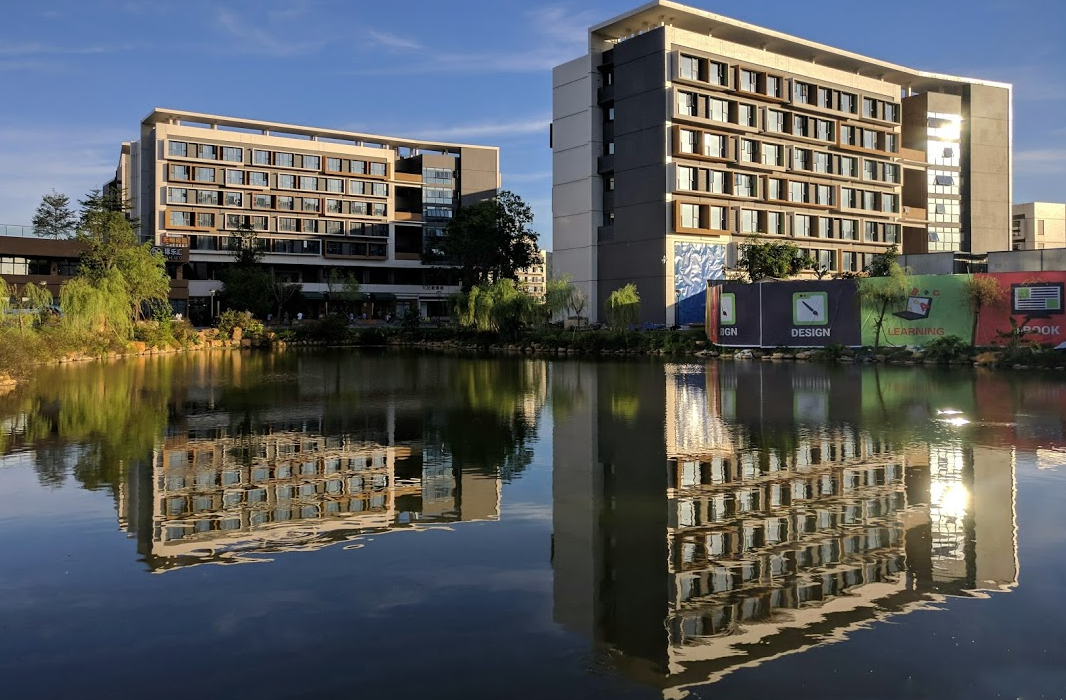
\includegraphics[scale=0.2]{assets/uic-landscape.png}
    \caption{External Picture Example: Landscape of BNU-HKBU UIC}
    \label{uic_landscape_picture}
\end{figure}
\subsection{Subsections}
Subsections are usually go to second or third levels in depth. This is heading 2 section.
\subsubsection{Heading 3 section}
This is heading 3 section.
\subsubsection{More sections}
If there are more sections, it is not suggested that more numbering levels are used. We can use the following way in give the fourth level section.
\subsection{\LaTeX~Functionality Demo}
\paragraph{Math Equation}
\begin{equation}
    \frac{1}{\displaystyle 1+
    \frac{1}{\displaystyle 2+
    \frac{1}{\displaystyle 3+x}}} +
    \frac{1}{1+\frac{1}{2+\frac{1}{3+x}}}
\end{equation}


\section{Fonts and Format and Binding}
The font is Times New Roman. The font size for text is 12 pt. The font size is 16 pt for heading 1 and 14 pt for heading 2. The main text must be justify-aligned. The left, right margin is 2 cm around and the top, bottom margin is 2.5 cm around. The students should prepare two hard copies, one is sent to the supervisor, and anther is sent to the FYP coordinator. Besides this, each student should also send a soft copy to supervisor.\cite{Gusfield:97}\par

\section{Reference, Citation and Conclusion}
Each thesis must offer the references materials in the end. For all the references, they are supposed to be cited somewhere in the thesis.\\
The work in the thesis should be summarized and put in the conclusion part.\cite{APA:83}

\phantomsection
\bibliography{fypref}
\bibliographystyle{ieeetr}

\phantomsection
\section*{Appendices (optional)}
\addcontentsline{toc}{section}{Appendices}
If there is anything that is offered to support the thesis but is not appropriate to appear in main text, it can be put there.


\end{document}